\Chapter{DNS y correo electrónico}\label{chap:4}

Esta práctica se centra en el uso de los protocolos de DNS y correo electrónico.

En una primera sección, se estudia el uso del protocolo DNS para resolver nombres de dominios.

En la última sección, se utilizan los protocolos SMPT y POP3 para enviar y recibir correos electrónicos.
En esta sección, se utiliza tanto el servidor de \verb#GMAIL# como el de uniovi para realizar las pruebas.
Utilizar el servidor de uniovi impone la necesidad de realizar esta práctica en la universidad,
ya que este servidor no es accesible desde fuera de la misma (a menos que se utilice una VPN).

\section{DNS}

El servicio DNS se encarga de resolver nombres de dominios.
El uso más general consiste en recibir un nombre de dominio y retornar su dirección IP.
No obstante, existen casos en los que se puede buscar la operación inversa u
otros datos sobre un nombre de dominio.

\subsection{Herramientas de línea de comandos}

Nos introducimos al uso de las herramientas de comandos más comunes a la hora de trabajar con DNS.
Estas herramientas muestran un distinto grado de granularidad en la información que presentan.

\subsubsection{nslookup}

La herramienta \verb#nslookup# nos retorna la dirección IP del servidor que estmos buscando
junto con información extra como el nombre canónico o la dirección IPv6.

\begin{minipage}{\linewidth}
	\centering
	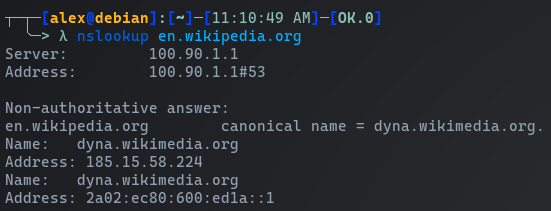
\includegraphics[width=0.8\textwidth]{4/Imagen41.png}
	\captionof{figure}{nslookup de en.wikipedia.org}\label{fig:4/1}
\end{minipage}

\subsubsection{host}

La herramienta \verb#host# retorna menos información que \verb#nslookup#,
simplemnete nos muestra la dirección IPv4 e IPv6 del servidor que buscamos. 
Esta herramienta tiene sin lugar a dudas la salida más legible (por un usuario) de las 3.

\begin{minipage}{\linewidth}
	\centering
	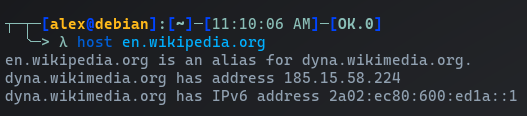
\includegraphics[width=0.8\textwidth]{4/Imagen42.png}
	\captionof{figure}{host de en.wikipedia.org}\label{fig:4/2}
\end{minipage}

\subsubsection{dig}

Finalmente, la herramienta \verb#dig# tiene la salida más barroca de las 3,
nos muestra información como el nombre canónico, la dirección IPv4 y
nos muestra también el servidor DNS que dio la respuesta entre otra información.

\begin{minipage}{\linewidth}
	\centering
	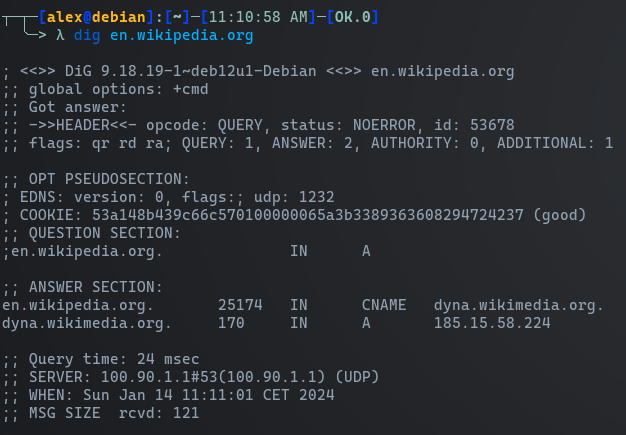
\includegraphics[width=0.8\textwidth]{4/Imagen43.png}
	\captionof{figure}{dig de en.wikipedia.org}\label{fig:4/3}
\end{minipage}

\subsubsection{en.wikipedia.org - es.wikipedia.org}

Comparamos la salida de \verb#nslookup# al buscar la dirección IP de los nombres
\verb#en.wikipedia.org# y \verb#es.wikipedia.org#.

\begin{minipage}{\linewidth}
	\centering
	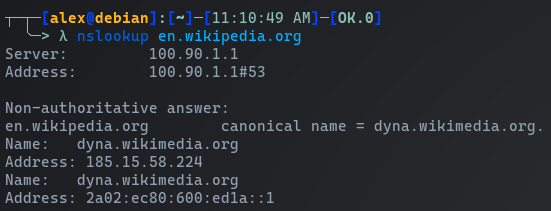
\includegraphics[width=0.8\textwidth]{4/Imagen41.png}
	\captionof{figure}{nslookup de en.wikipedia.org}\label{fig:4/4}
\end{minipage}

\begin{minipage}{\linewidth}
	\centering
	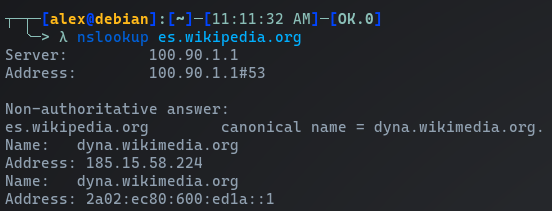
\includegraphics[width=0.8\textwidth]{4/Imagen44.png}
	\captionof{figure}{nslookup de es.wikipedia.org}\label{fig:4/5}
\end{minipage}

Como podemos ver, ambas consultas retornan la misma información,
en ambos casos el nombre se resuelve a la dirección IP \verb#185.15.58.224#
o \verb#2a02:ec80:600:ed1a::1# en el caso de IPv6.

\subsubsection{DNS 8.8.8.8}

La dirección del servidor DNS preferido puede ser modificada en el fichero \verb#/etc/resolv.conf#.
Insertamos la direción \verb#8.8.8.8# en la primera linea de este fichero para que este sea el servidor con
mayor prioridad.

\begin{minipage}{\linewidth}
	\centering
	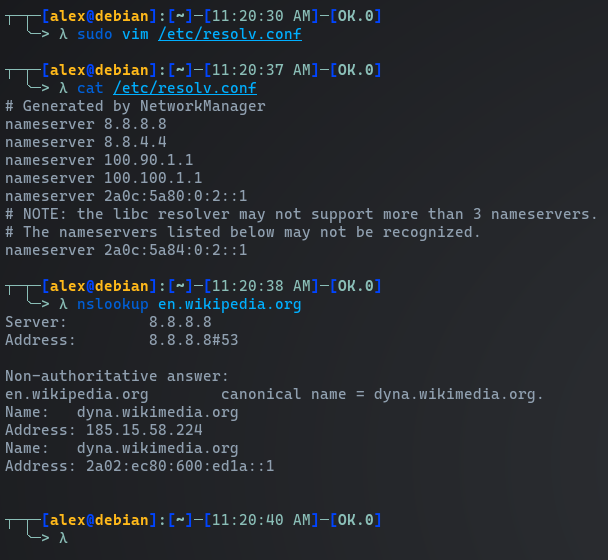
\includegraphics[width=0.8\textwidth]{4/Imagen45.png}
	\captionof{figure}{Modificación de /etc/resolv.conf}\label{fig:4/6}
\end{minipage}

Como podemos ver, al hacer la consulta de cualquier nombre
obtenemos la misma respuesta es la misma dirección IP,
pero el servidor que está respondiendo ha pasado a ser el \verb#8.8.8.8#.

\subsection{Búsqueda iterativa}

En esta sección buscamos la dirección IP del servidor \verb#en.wikipedia.org#,
comenzando desde un servidor DNS raiz.

\subsubsection{Consulta sobre dominio raíz}

Al consultar al servidor \verb#8.8.8.8# sobre el dominio raíz,
obtenemos el nombre \verb#a.root-servers.net# en el campo \verb#SOA#.

Procedemos a consultar sobre la IP de este servidor:

\begin{minipage}{\linewidth}
	\centering
	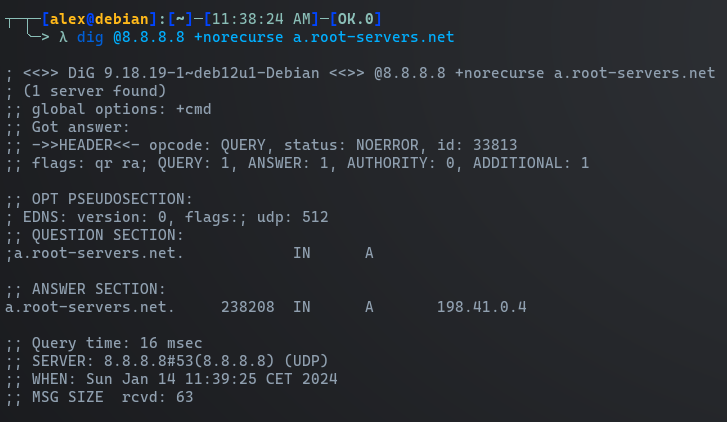
\includegraphics[width=0.8\textwidth]{4/Imagen48.png}
	\captionof{figure}{Consulta sobre DNS a.root-servers.net}\label{fig:4/7}
\end{minipage}

En la respuesta, observamos que la dirección IPv4 de este servidor es
\verb#198.41.0.4# (campo \verb#A#).

\subsubsection{Consulta sobre .org}

Utilizamos el nuevo servidor para consultar sobre el dominio \verb#.org#:

\begin{minipage}{\linewidth}
	\centering
	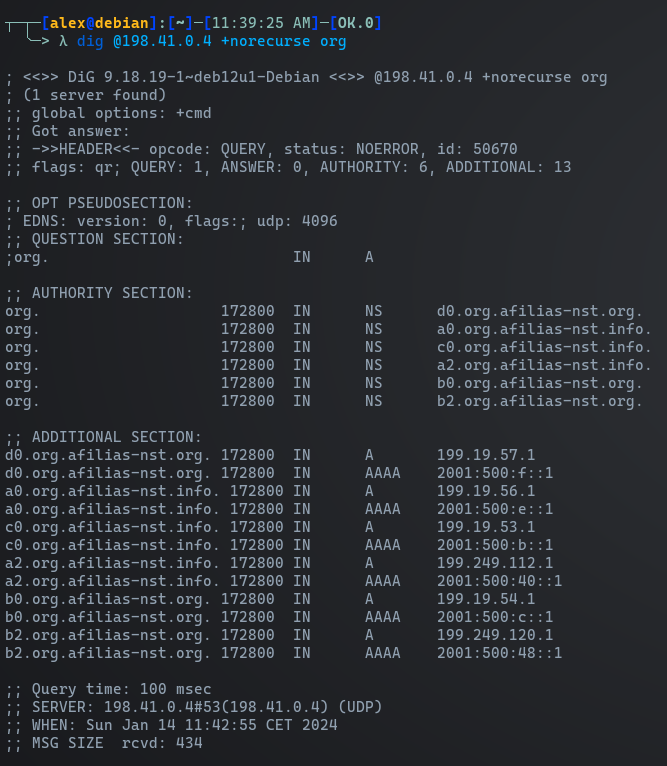
\includegraphics[width=0.8\textwidth]{4/Imagen49.png}
	\captionof{figure}{Consulta sobre dominios .org}\label{fig:4/8}
\end{minipage}

Obtenemos múltimples servidores, escogemos uno de ellos.
En este caso, hemos escogido el servidor \verb#d0.org.afilias-nst.org#
con dirección IPv4 \verb#199.19.57.1#.

\subsubsection{Consulta sobre wikipedia.org}

Utilizamos el nuevo servidor para consultar sobre el dominio \verb#wikipedia.org#:

\begin{minipage}{\linewidth}
	\centering
	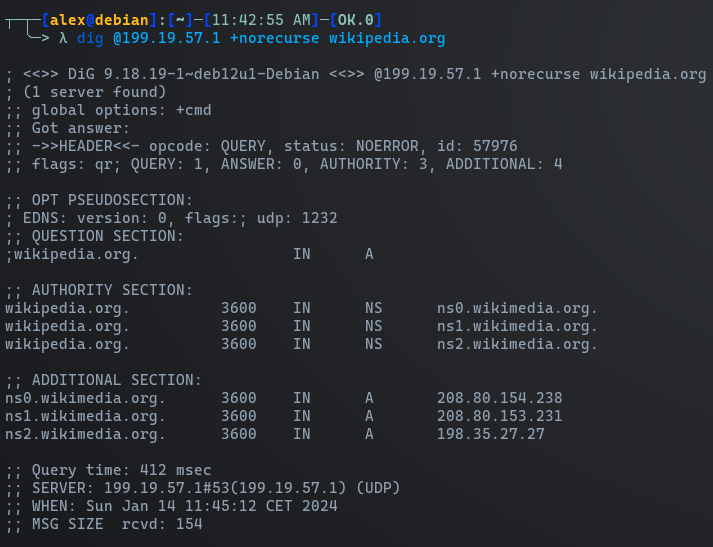
\includegraphics[width=0.8\textwidth]{4/Imagen491.png}
	\captionof{figure}{Consulta sobre wikipedia.org}\label{fig:4/9}
\end{minipage}

Obtenemos 3 servidores de wikipedia, escogemos cualquiera de ellos.
En este caso, hemos escogido el servidor \verb#ns0.wikimedia.org#
con dirección IPv4 \verb#208.80.154.238#.

\subsubsection{Consulta sobre en.wikipedia.org}

Utilizamos el nuevo servidor para consultar sobre el dominio \verb#en.wikipedia.org#:

\begin{minipage}{\linewidth}
	\centering
	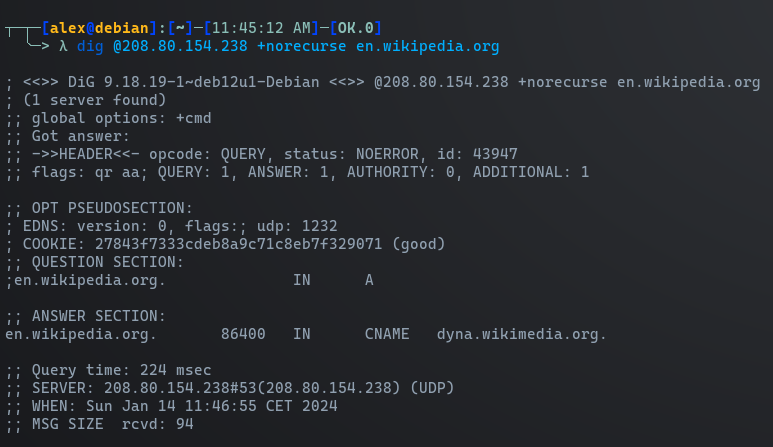
\includegraphics[width=0.8\textwidth]{4/Imagen492.png}
	\captionof{figure}{Consulta sobre en.wikipedia.org}\label{fig:4/10}
\end{minipage}

Esta consulta no nos retorna una dirección IP,
sino que nos retorna un CNAME (\verb#dyna.wikimedia.org#).
Consultamos sobre este CNAME al mismo serviodor:

\begin{minipage}{\linewidth}
	\centering
	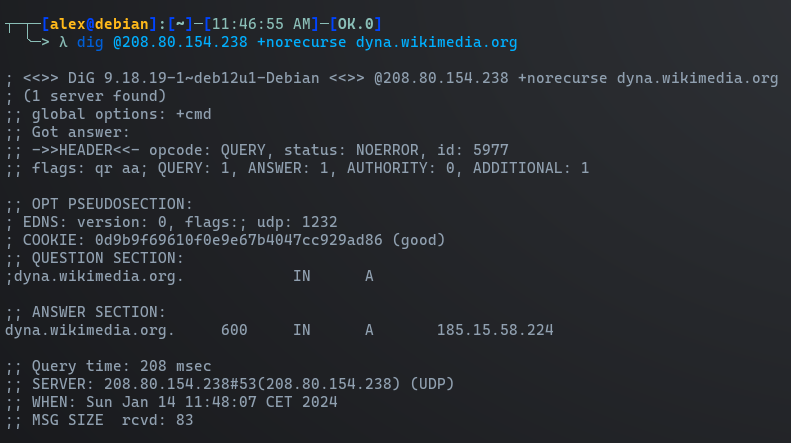
\includegraphics[width=0.8\textwidth]{4/Imagen493.png}
	\captionof{figure}{Consulta sobre dyna.wikimedia.org}\label{fig:4/11}
\end{minipage}

Finalmente, obtenemos la dirección IP \verb#185.15.58.224#
que coincide con la dirección IP que obteníamos en secciones
anteriores al consultar sobre este nombre de dominio.

\subsection{DNS desde el programa (Python)}

Utilizamos la librería \verb#dnspython# para escribir un programa que
dado un nombre de dominio retorne su dirección IP.

\begin{minipage}{\linewidth}
	\centering
	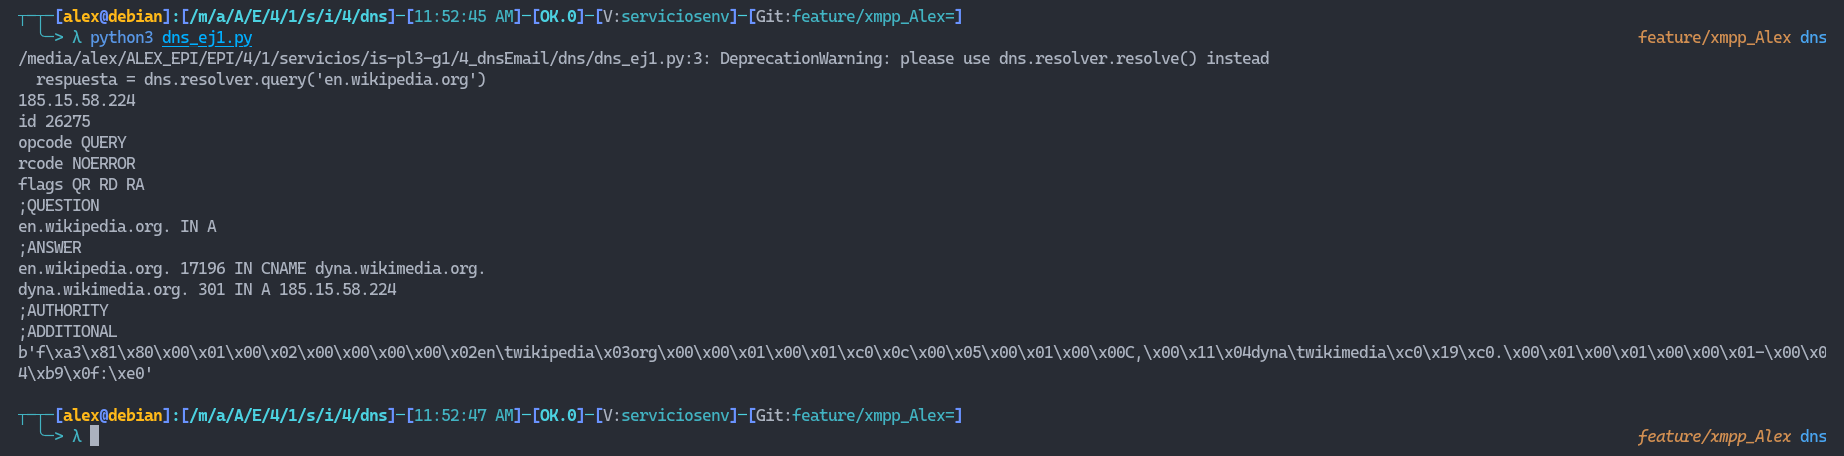
\includegraphics[width=0.8\textwidth]{4/Imagen494.png}
	\captionof{figure}{dnspython}\label{fig:4/12}
\end{minipage}

Al consultar por \verb#apple.com#, obtenemos sólo una dirección IP.

\begin{minipage}{\linewidth}
	\centering
	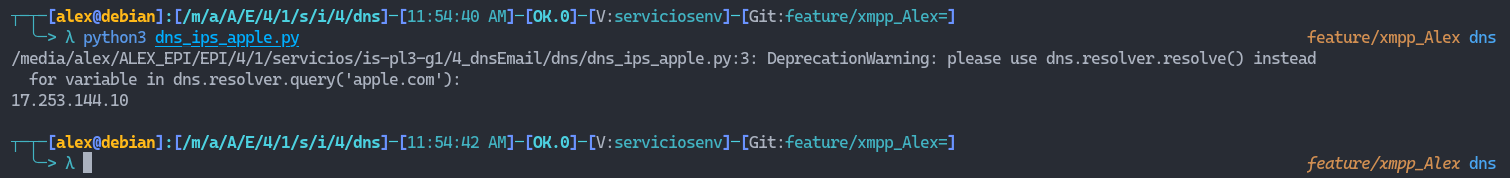
\includegraphics[width=0.8\textwidth]{4/Imagen495.png}
	\captionof{figure}{IP de apple.com}\label{fig:4/13}
\end{minipage}

\subsection{API POSIX (OPCIONAL)}

\section{Correo Electrónico}

\subsection{Envío de correo}

El sistema de correo electrónico utiliza códigos de retorno para confirmar
al cliente el estado actual de la transacción.

A diferencia de HTTP, donde el código 200 implica que todo procede correctamente,
en SMPT cada mensaje retorna un código de confirmación diferente.

Esto implica que para cada mensaje que se envia, el cliente tiene que esperar un
número distinto.

\begin{notebox}
    Al enviar \verb#HELO#, el servidor retorna \verb#250# si todo procede correctamente.\\
    Pero al enviar \verb#DATA\r\n#, el servidor retorna \verb#354# si todo procede correctamente.
\end{notebox}

Por ello, hemos decidido almacenar los mensajes en pares,
de forma que cada mensaje vaya acompañado por su código de retorno esperado.

\subsection{Envío de correo seguro (SSL)}

A continuación, utilizamos el servidor de correo de \verb#GMAIL# para enviar correos electrónicos.
Para ello, es necesario crear una clave de aplicación.

Esta es la salida del programa al ser ejecutado.
Se envía un email entre nuestras cuentas personales de gmail.

\begin{minipage}{\linewidth}
	\centering
	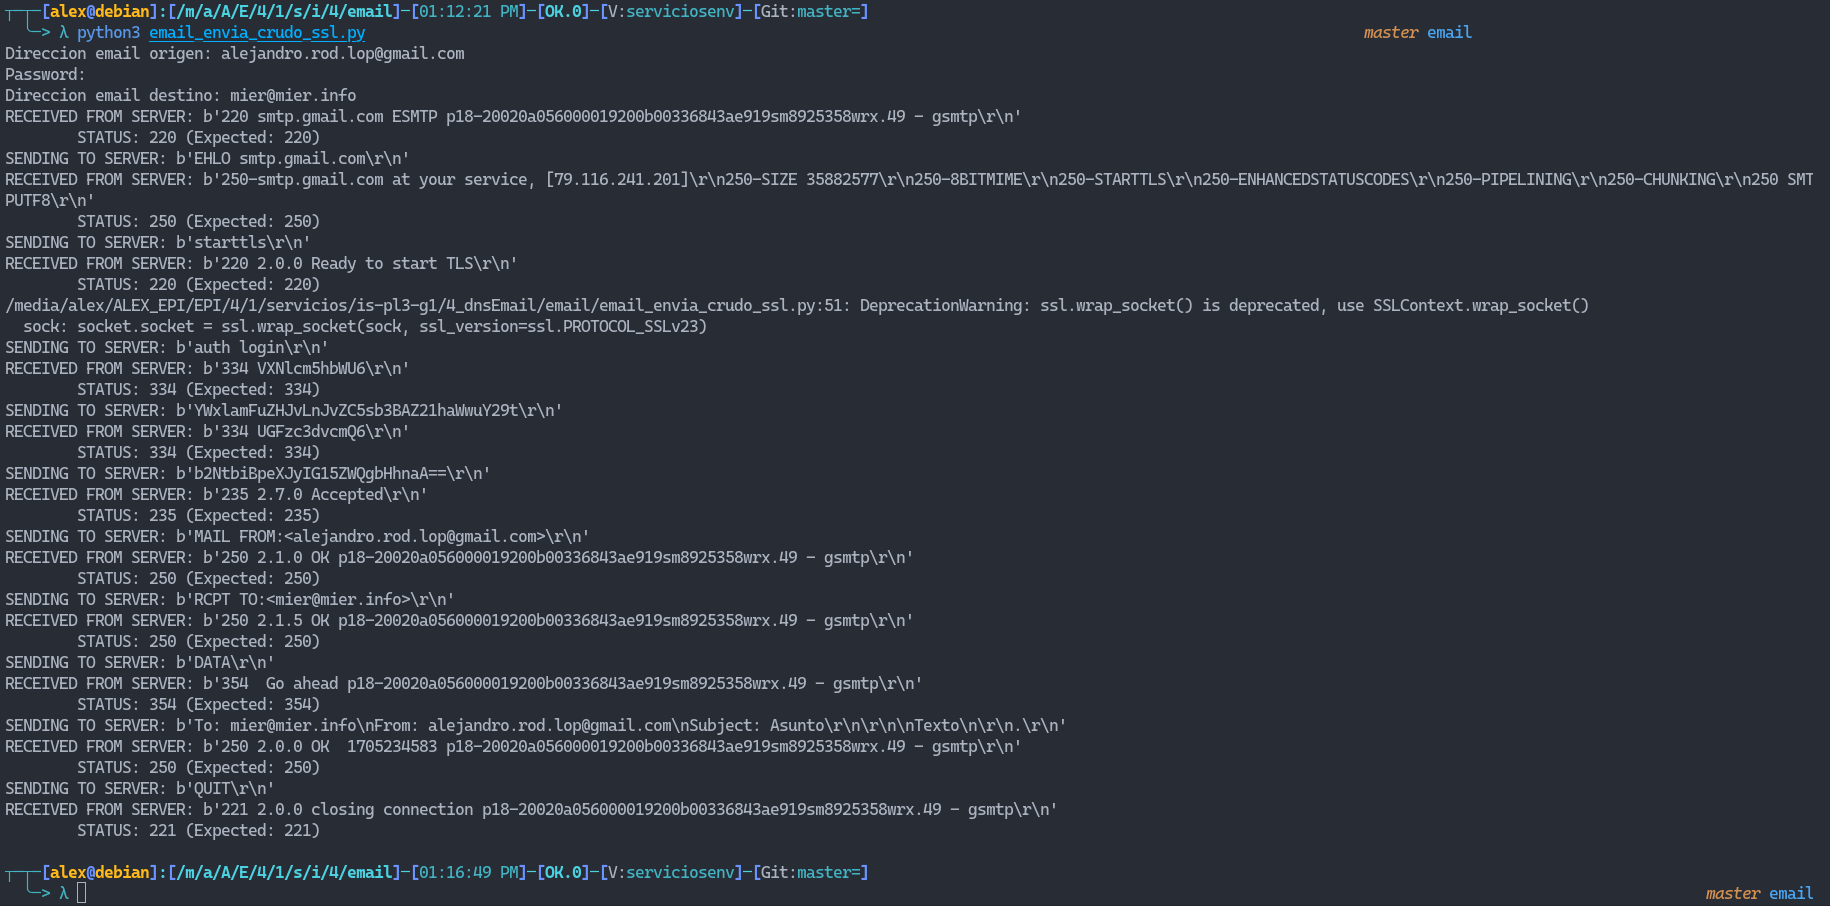
\includegraphics[width=0.8\textwidth]{4/Imagen496.png}
	\captionof{figure}{Envío correo electrónico GMAIL}\label{fig:4/14}
\end{minipage}

El correo recibido en la cuenta del receptor.

\begin{minipage}{\linewidth}
	\centering
	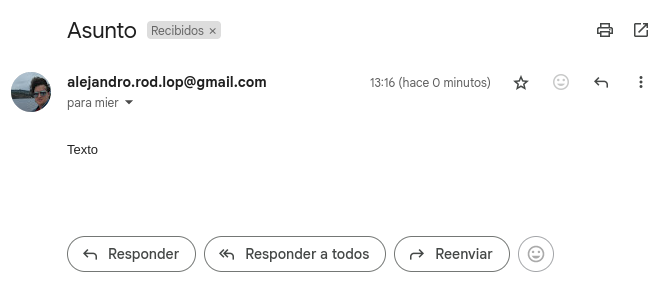
\includegraphics[width=0.8\textwidth]{4/correo.png}
	\captionof{figure}{Correo recibido desde el destinatario}\label{fig:4/15}
\end{minipage}

\subsection{Lectura de correo (POP3)}

Escribimos un programa que lea los correos sin leer de una cuenta de \verb#GMAIL#.
De esos mensajes, extrae el asunto y el remitente.

A continuación se muestra una captura de pantalla de lo retornado por el programa.

\begin{minipage}{\linewidth}
	\centering
	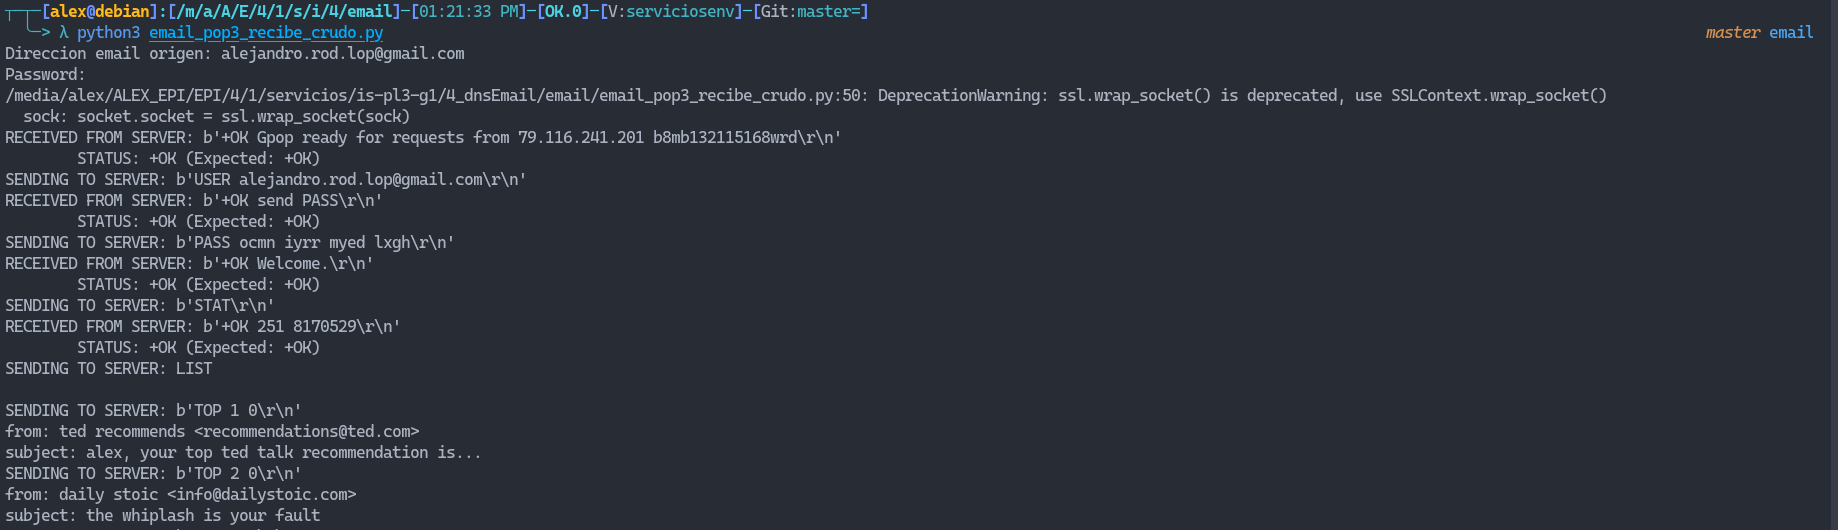
\includegraphics[width=0.8\textwidth]{4/Imagen497.png}
	\captionof{figure}{Remitentes y asuntos de correos sin leer}\label{fig:4/16}
\end{minipage}

Finalmente, utilizamos la librería \verb#poplib# para recibir los mensajes de correo.
Al ejectuar nuestro programa básico obtenemos una salida que contiene todos los emails
sin leer.

A continuación se muestra parte de la salida.

\begin{minipage}{\linewidth}
	\centering
	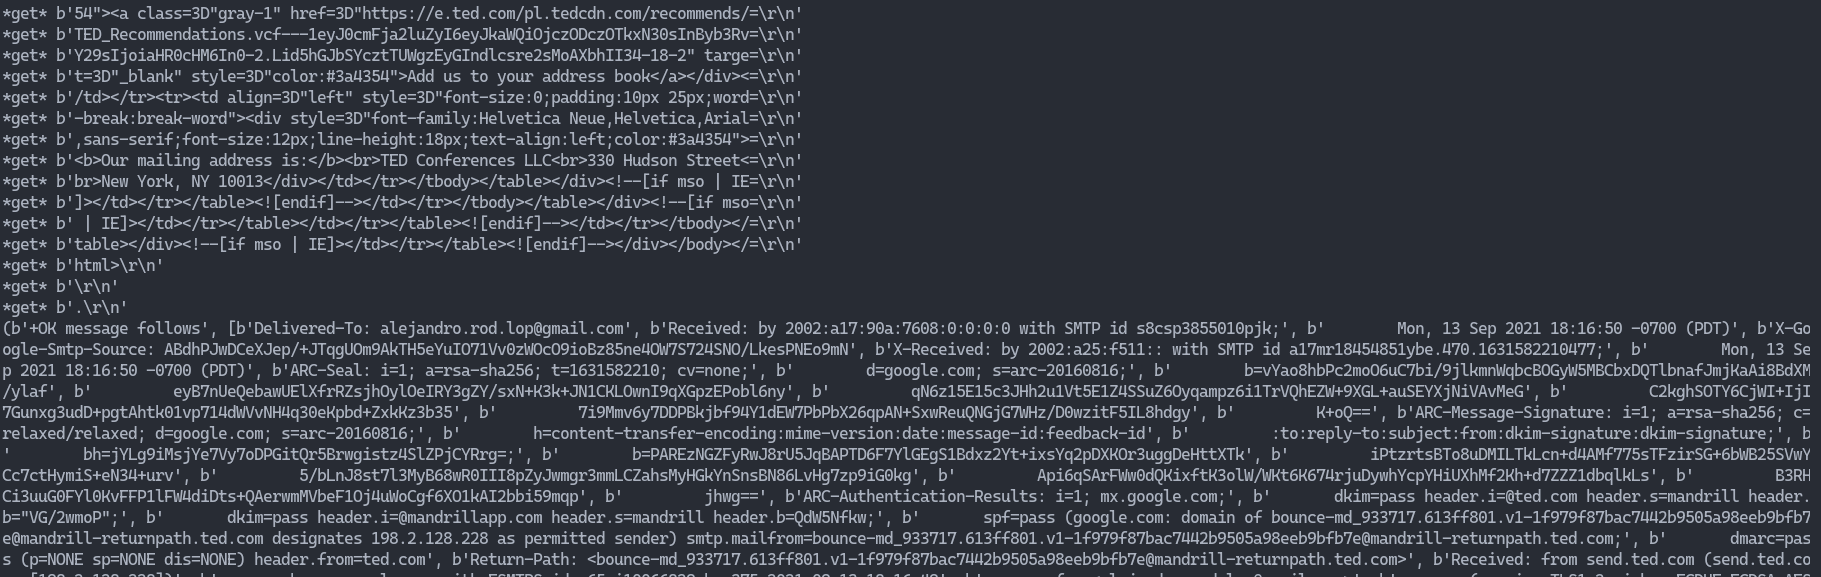
\includegraphics[width=0.8\textwidth]{4/Imagen498.png}
	\captionof{figure}{Salida de poplib}\label{fig:4/17}
\end{minipage}
